\documentclass{article}

% stations weg, heb het alleen over receivers. Een station is dan ook gewoon een receiver

%% polarisaties weg halen.
%% Wel uitleggen dat ze er zijn, maar voor de filters en de correlator
%% zijn het gewoon onafhankelijke receivers. Dit maakt de pseudo code + optimalisaties veel compacter.
% @@@ Rob: dit klopt helemaal niet. Voor de polarisaties moet je namelijk ALLE combinaties uitrekenen.
% DUS zowel XY als YX. Voor stations doe je dit niet. We kunnen polarisaties dus niet weg laten.
% Daarom kwam John ook op een AI van 0.5 uit IPV 1.


% opencl uitzoeken
%  - hoe gaat opencl om met random writes?
% RANDOM WRITES ZIJN GEWOON TOEGESTAAN.

% uitzoeken: andere toepassingen van correleren: geofysica? radar? wifi 802.11n, wimax???



% zoek parallelisme: onafhankelijke berekeningen
% voor de correlator geldt dat de berekiningen onafhankelijk zijn, maar IO niet!
% met many cores is de I/O vaak de bottleneck


%% pas je algorithmen aan op many-cores


%% 1) zoek parallelisme in je algorithme.
%%    vaak aanwezig. Zoek onafhankelijke operaties:
%%     voorbeelden:
%%    - correlator: kanalen, polatisaties, subbanden zijn onafhankelijk.
%%    - polyphase: stations zijn onafhankelijk
%%    - imaging: maak parallelisme: beeld elk kanaal af op een image, tel deze later op

  
%% 2) mem bw/ops neemt af met many cores
%%    optimaliseer.

%% dus optimaliseren: 
%%     - algo specifiek (reduceer mem loads)
%%     - architectuur-specifieke optimalisaties (cache gedrag, delays, floating point instructions)


\usepackage{spconf}
\usepackage{graphicx}
\usepackage{listings}


\newcommand{\longversion}[1]{}
\newcommand{\shortversion}[1]{#1}

\title{How to Build a Correlator with Many-Core Hardware}

\name{Rob V. van Nieuwpoort and John W. Romein}

\address{Stichting ASTRON (Netherlands Institute for Radio Astronomy) \\
Oude Hoogeveensedijk 4, 7991 PD\ \ Dwingeloo, The Netherlands \\
\texttt{\{nieuwpoort,romein\}@astron.nl}
}


\begin{document}

\maketitle

\begin{abstract}
A recent development in radio astronomy is to replace traditional dishes
with many small antennas. The signals are combined to form one large,
virtual telescope.  The enormous data streams are cross-correlated to
filter out noise.  A recent trend is to correlate in software instead of dedicated hardware. Examples
include e-VLBI and LOFAR.
In this paper, we explain how to implement and optimize a correlator 
 on multi-core CPUs
and many-core architectures, such as NVIDIA and ATI GPUs,
and the \mbox{Cell/B.E.}  The correlator is a streaming, real-time
application, and is much more I/O intensive than applications that are
typically implemented on many-core hardware today.  We compare with
the LOFAR production correlator on an IBM Blue Gene/P supercomputer.
We identify several important architectural problems which cause
architectures to perform suboptimally, and also deal with programmability. 
Our findings are applicable to signal processing applications in general.

The results show that the processing power and memory bandwidth of
current GPUs are highly imbalanced.  While
the production correlator on the Blue Gene/P achieves a superb 96\% of the
theoretical peak performance, this is only 14\% on ATI GPUs, and 26\%
on NVIDIA GPUs. The \mbox{Cell/B.E.} processor, in contrast, achieves an
excellent 92\%. The research presented is an
important pathfinder for next-generation telescopes.
\end{abstract}

\section{Introduction}
% wat gaat de lezer leren van dit paper?

% we geven een leidraad voor het kiezen van de juiste architectuur voor het probleem van de lezer
% voor goede performance heb je nodig:
%  - kennis van algorithme
%  - kennis van de architecturen
%  - inzicht over hoe je de mapping van algorithme op architectuur het beste kunt doen
% dit paper geeft inzicht in de verschillen tussen architecturen, en inzicht over welke factoren belangrijk zijn om de mapping goed te doen.

Radio telescopes produce enormous amounts of data.
The Low Frequency Array, for instance, will produce some tens of
petabits per day, and the Australian SKA Pathfinder will
even produce over six exabits per day.
These modern radio telescopes use many separate receivers as building blocks, and
combine their signals to simulate a single large and sensitive instrument.
To extract the sky signal from the system noise, the \emph{correlator\/}
correlates the signals from different receivers, and integrates the correlations over time, to reduce
the amount of data. The correlation is an important problem in radio astronomy,
since the data volumes are so large, and the computational demand grows quadratically
with the number of receivers.

Traditionally, custom-built hardware is used to correlate the signals.
A recent development is to use a supercomputer~\cite{Romein:06}.
Both approaches have important advantages and disadvantages.
Custom-built hardware is efficient and consumes modest amounts of power, but is
inflexible, expensive to design, and has a long development time.
Solutions that use a supercomputer are much more flexible, but are less
efficient, consume more power, and are expensive to purchase and maintain.
Future instruments, like the Square Kilometre Array (SKA), need several orders
of magnitude more computational resources.
It is likely that the requirements of the SKA cannot be met by using
current supercomputer technology. Therefore, it is important to investigate
alternative hardware solutions, in particular the many-core architectures.

A recent development is that general-purpose architectures no longer
achieve performance increases by increasing the clock frequency, but
by adding more compute cores and exploiting parallelism.  Intel's
recent core~i7 processor is a good example of this. It has four
compute cores, but eight concurrent threads can be used thanks to the
hyperthreading technique. In addition, the cores can exploit vector
parallelism with the SSE instruction set.

Furthermore, the high-performance computing community is
steadily adopting clusters of Graphics Processor Units (GPUs) as a viable
alternative to supercomputers, due to their unparalleled growth in
computational performance, increasing flexibility, increasing programmability,
high power efficiency, and low purchase costs.
High-end GPUs are highly parallel and contain hundreds of processor cores.
%% However, their usefulness is often limited to applications that do not require
%% double-precision floating-point arithmetics, since there is no need for
%% double-precision calculations to play games.
%% Hence, the support for double-precision arithmetic is typically poor.
%% Fortunately, many signal-processing applications do not require double
%% precision.

The IBM Cell Broadband Engine~\cite{cell}, well known from the
PlayStation~3, is another example of a processor that combines GPU and CPU
qualities into one design.
The Cell/B.E. consists of an ``ordinary'' PowerPC core and eight powerful
vector processors with fast, local memories that provide
the bulk of the processing power.
Programming the Cell/B.E. requires more effort than programming an ordinary CPU,
but various studies showed that the Cell/B.E. performs very well on
signal-processing tasks like FFTs~\cite{fftc}.

In this article, we explain how modern multi-core architectures can be
exploited for signal-processing purposes.  Additionally, we give
insights into their architectural limitations, and how to best cope
with them.  We treat five different, popular architectures with
multiple cores: the IBM Cell/B.E., GPUs from both NVIDIA and ATI, the Intel Core i7 processor, and
the IBM Blue Gene/P supercomputer.  We discuss their
similarities and differences, and how the architectural differences
affect optimization choices and the eventual performance of a
correlator.  We strongly focus on correlators, but many of the
findings, claims, and optimizations hold for other signal-processing
algorithms as well, both in and outside the area of radio astronomy.
We discuss the programmability of each of the architectures, but this
paper should be of special interest to those who are willing to invest
some extra programming effort to obtain good performance, even if
high-level programming support is not available.

In this paper, we use the LOFAR telescope as a running example, and
use the production correlator on the Blue Gene/P as a comparison. This way,
we can demonstrate how many-core architectures can be used in practice for a real
application. Nevertheless, the results apply equally well to other
instruments and applications.


\section{Trends in radio astronomy}

%% @@@
%% It is important that the authors take a tutorial 
%% oriented style and more carefully introduce the 
%% application context, including radio-astronomy 
%% basics, instruments that they use (including 
%% installation roadmap).  The algorithm is quite 
%% simple and so the strength of the paper lies in 
%% the thoroughness of the analysis, and the 
%% aforementioned tutorial background.
%% @@@

%- signal processing neemt een dominantere rol (meer antennes, etc)
%- voorbeelden. pathfinders voor SKA. 
%- computationally intensive, SKA even more

%@@@ later even kijken: computing advances maken nieuwe signal processing technieken en telescopen / instrumenten mogelijk.



During the past decade, new types of radio-telescope concepts emerged that
rely less on concrete, steel, and extreme cooling techniques, but more on
signal-processing techniques.
For example, LOFAR~\cite{Butcher:04} is a distributed sensor network
that combines the signals of tens of thousands of simple receiver elements.
Other examples are MeerKAT (Karoo Array Telescope)~\cite{meerkat} and
ASKAP (Australian Square Kilometre Array Pathfinder)~\cite{askap}. Both are
pathfinders for the future SKA (Square Kilometre Array)~\cite{ska} telescope, which
will be orders of magnitude larger.
Also, Aperture Array tiles like Embrace~\cite{embrace} and Focal Plane Arrays
like Apertif~\cite{apertif} are novel multi-receiver concepts.
Unlike single-pixel feeds from traditional dish-based telescopes, these
concepts combine the advantages of higher sensitivity, higher resolution,
and multiple, concurrent observation directions.
What the noveal instruments all have in common is that they require huge
amounts of processing power to combine the data from the receiving elements.

The signal-processing hardware technology used to process telescope
data also changes rapidly.  Only a decade ago, correlators required
special-purpose ASICs to keep up with the high data rates and
processing requirements.  The advent of sufficiently fast FPGAs
significantly lowered the developments times and costs of
newer-generation correlators, and increased the flexibility
substantially. LOFAR requires even more flexibility to support many
different processing pipelines for various observation modes, and uses
FPGAs for on-the-field processing and a Blue Gene/P
supercomputer to perform real-time, central processing.
We describe LOFAR in more detail below.

%  dit past hier niet
%% Recent many-core architectures seem to be a viable complement to the aforementioned processing platforms.
%% GPUs provide more processing power and are more power-efficient than CPUs,
%% while GPUs are more flexible and easier to program than FPGAs.
%% Since GPUs of different vendors are mutually quite different, we did an
%% extensive performance comparison between the architectures of popular GPUs 
%% for signal-processing purposes, particularly, for correlation
%% purposes~\cite{Nieuwpoort:09}.


\subsection{The LOFAR telescope}

\begin{figure}[ht]
\begin{center}
\includegraphics[width=60mm]{figures/LBA-field.jpg}
\end{center}
\caption{A field with LOFAR antennas.}
\label{fig:lba-field}
\end{figure}

\begin{figure*}
\begin{minipage}[b]{11cm}
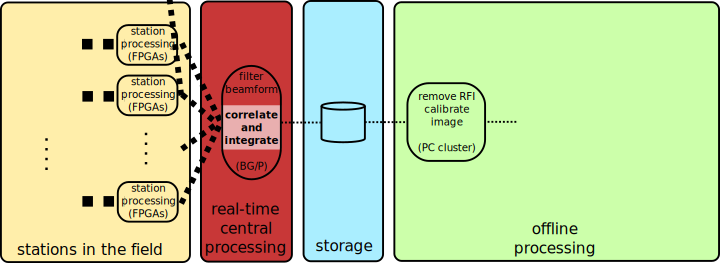
\includegraphics[width=11cm]{figures/lofar-overview.pdf}
\caption{A simplified overview of the LOFAR processing.}
\label{fig:lofar-overview}
\end{minipage}
\hfill
\begin{minipage}[b]{56mm}
\includegraphics[width=\columnwidth]{figures/map.jpg}
\caption{Possible LOFAR layout.}
\label{fig:map}
\end{minipage}
\end{figure*}

LOFAR is an acronym for \emph{\textbf{LO}w \textbf{F}requency
  \textbf{AR}ray}, an aperture array radio telescope operating in the
10 to 250~MHz frequency range~\cite{Butcher:04}.  It is the first of a new generation of
radio telescopes, that breaks with the concepts of traditional
telescopes in several ways.  Rather than using large, expensive
dishes, LOFAR uses many thousands of simple antennas that have no
movable parts, see
Figure~\ref{fig:lba-field}.  Essentially, it is a distributed sensor
network that monitors the sky and combines all signals centrally.
This concept requires much more signal processing, but the 
costs of the silicon for the processing are much lower that the costs of steel that would
be needed for dishes. Moreover, LOFAR can observe the sky in many
directions concurrently and switch directions instantaneously.  In
several ways, LOFAR will be the largest telescope of the world.

Another novelty is the elaborate
use of \emph{software\/} to process the telescope data in real time.
The signals from the
antennas are digitised, transported to a central location,
and combined in software to emulate a conventional antenna. 
LOFAR thus is an IT-telescope. 
The cost
is dominated by the cost of electronics and will follow Moore's law,
becoming cheaper with time and allowing increasingly large telescopes
to be built. 

The antennas are simple, but there are a lot of them: 25000 in the full LOFAR
design. To make radio pictures of the sky with adequate sharpness,
these antennas are to be arranged in clusters that are spread out over
an area of ultimately 350 km in diameter. This is shown in Figure~\ref{fig:map}.
In the current phase, 15000 
antenna's and maximum baselines of 100 km will
be built. Data transport requirements are in the range of many
Tera-bits/sec and the processing power needed is tens of Tera-FLOPS.

LOFAR will enable exciting new science cases.  First, we expect to see
the \emph{Epoch of Reionization\/} (EoR), the time that the first star
galaxies and quasars were formed. Second, LOFAR offers a unique
possibility in particle astrophysics for studying the origin of
high-energy \emph{cosmic rays}.  Third, LOFAR's ability to
continuously monitor a large fraction of the sky makes it uniquely
suited to find new \emph{pulsars} and to study \emph{transient
  sources}.  Since LOFAR has no moving parts, it can instantaneously
switch focus to some galactic event.  Fourth, \emph{Deep Extragalactic
  Surveys\/} will be carried out to find the most distant radio
galaxies and study star-forming galaxies.  Fifth, LOFAR will be
capable of observing the so far unexplored radio waves emitted by
\emph{cosmic magnetic fields}.  For a more extensive description of
the astronomical aspects of the LOFAR system, see De Bruyn
et.~al.~\cite{Bruyn:02}.

A global overview of the LOFAR processing is given in
Figure~\ref{fig:lofar-overview}. The thickness of the lines indicates
the size of the data streams.  Initial processing is done in the
field, using FPGA technology.  Typical operations that are performed
there include analog-to-digital conversion, filtering, frequency
selection, and combination of the signals from the different
receivers.  Next, the data is transported to the central processing
location in Groningen via a Wide-Area Network (WAN), using owned and
leased light paths.

Currently, the real-time central processing of LOFAR data is done on
an IBM Blue Gene/P supercomputer.  There, we filter the data, and
perform phase shift and bandpass corrections, and beam forming.
Finally, the signals from all stations are cross-correlated.  The
correlation process performs a data reduction by integrating samples
over time.  Finally, the data is forwarded to a storage cluster, where
results can be kept for several days.  After an observation has
finished, further processing is done off-line, on commodity cluster
hardware.  In this paper, we focus on the correlator step (the
highlighted part in the red box in
Figure~\ref{fig:lofar-overview}), because it must deal with the
full data streams from all receivers. Moreover, its costs grow
quadratically with the number of receivers, while all other steps have
a lower time complexity.


\section{Correlating signals}



%XF vs FX. lofar is FX. Met een groter aantal inputs is FX efficienter?
%transpose


%% \begin{figure*}[t]
%% \begin{center}
%% 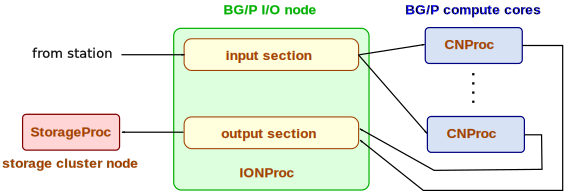
\includegraphics[width=12cm]{figures/processing-overview.pdf}
%% \end{center}
%% \vspace{-0.5cm}
%% \caption{A simplified view of LOFAR processing.}
%% \label{fig-processing-overview}
%% \end{figure*}


The data streams from the receivers contain samples, which are complex
numbers that represent the amplitude and phase of a signal at a
particular time.  The receivers are dual-polarized; they take separate
samples from orthogonal (X and Y) directions.  The LOFAR receivers
support 4, 8 and 16 bit integer samples, where the normal mode of
operation uses the 16 bit samples. The smaller 4 and 8 bit samples are important
for observations that require larger frequency bands, but with less accuracy.
The future SKA telescope will
likely use 2 bit samples.  Before filtering and correlating, the
samples are converted to single precision floating point.  This is
accurate enough for our purposes. From the perspective of the
correlator, samples thus consist of \emph{four} 32-bit floating point
numbers: two polarizations, each with a real and an imaginary part.

Prior to correlation, the data that comes from
the receivers must be reordered:
each input carries the signals of many frequency bands from a single
receiver, but the correlator needs data from a single frequency of all inputs.
Depending on the data rate, switching the data can be a real challenge.
The data reordering phase is outside the scope of this paper, but a correlator
implementation cannot ignore this issue.
The LOFAR Blue Gene/P correlator uses the fast 3D~torus for this purpose;
other multi-core architectures need external switches.

The received signals from sky sources are so weak, that the antennas 
mainly receive noise. To see if there is statistical coherence
in the noise, simultaneous samples of each pair of receivers are correlated, 
by multiplying the sample of one receiver with the complex
conjugate (i.e., the imaginary part is negated) of the sample of the other receiver.
To reduce the output size, the correlations are integrated, by accumulating all products. 
Therefore, the correlator is mostly multiplying and adding complex numbers.
Both polarizations of a station A are correlated with both polarizations 
of a station B, yielding correlations in XX, XY, YX, and YY
directions.
The correlator algorithm itself thus is straightforward, and can be
written in a single formula: \\
$C_{s_1,s_2\geq s_1,p_1\in\{X,Y\},p_2\in\{X,Y\}} = \displaystyle\sum_{t} Z_{s_1,t,p_1} * Z_{s_2,t,p_2}^\ast$ 

The total number of correlations we have to compute is $(nrReceivers \times
(nrReceivers + 1)) / 2$, since we need each pair of correlations only
once. This includes the autocorrelations (the correlation of a receiver with itself),
since we need them later in the pipeline for calibration purposes.
The autocorrelations can be computed with half the number of instructions.

We can implement the correlation operation very efficiently, with only
four fused-multily-add (fma) instructions, doing eight floating-point
operations in total. For each pair of receivers, we have to do this
four times, once for each combination of polarizations. Thus, in total
we need 32 operations. To perform these operations, we have to load
the samples generated by two different receivers from memory.  As
explained above, the samples each consist of four single precision
floating point numbers (a real and imaginary part, and two
polarizations).  Therefore, we need to load 8 floats or 32 bytes in
total.  This results in \emph{exactly one FLOP/byte}.  The number of
operations that is performed per byte that has to be loaded from main
memory is called the \emph{arithmetic
  intensity}~\cite{system-performance}.  For the correlation
algorithm, the arithmetic intensity is extremely low.
We will describe the implementation and optimization of the correlator on the
many-core sytems in more detail in Section~\ref{sec:optimizing}, but first, we explain the architectures themselves. 


\section{Many-core architectures}

%TODO: zet kolommen in de volgorde van behandeling
\begin{table*}[t]
\begin{center}
{\footnotesize
\begin{tabular}{|l|l|l|l|l|l|}                                                   
\hline
Architecture                                 & Intel Core i7 & IBM Blue Gene/P& ATI 4870 &  NVIDIA Tesla C1060 & STI Cell/B.E. \\
\hline
\textbf{gflops per chip}                     & \textbf{85}   & \textbf{13.6}  & \textbf{1200}  & \textbf{936}  & \textbf{204.8}\\
Clock frequency (GHz)                        & 2.67          & 0.850          & 0.75           & 1.296         & 3.2           \\
cores x FPUs per core = \textbf{total FPUs}  & 4x4 = \textbf{16} & 4x2 = \textbf{8} & 160x5 = \textbf{800} & 30x8 = \textbf{240} & 8x4 = \textbf{32} \\
%operations per cycle per FPU                & 2             &   2            & 2              & 2             & 2             \\
%\hline
registers per core x register width          & 16x4          & 64x2           & 1024x4        & 2048x1         & 128x4         \\
%\hline
%total L1 data cache size per chip (KB)      & 32            & 128            & undisclosed   & undisclosed    & 2048          \\
%total L1 cache bandwidth (GB/s)             & undisclosed   & 54.4           & 480           & undisclosed    & 409.6         \\
total device RAM bandwidth (GB/s)            & n.a.          & n.a.           & 115.2         & 102            & n.a.          \\
\textbf{total host RAM bandwidth (GB/s)}     & \textbf{25.6} & \textbf{13.6}  & \textbf{8.0}  & \textbf{8.0}   & \textbf{25.8} \\
%\hline
%Process Technology (nm)                      & 45            & 90             & 55            & 65             & 65            \\
%TDP (W)                                      & 130           & 24             & 160           & 236            & 70            \\
%\textbf{gflops / Watt (based on TDP)}       & \textbf{0.65} & \textbf{0.57}  & \textbf{7.50} & \textbf{3.97}  & \textbf{2.93} \\
%\hline
%\textbf{gflops/device bandwidth (gflops / GB/s)}& n.a.       &  n.a.          & \textbf{10.4} & \textbf{9.2}   & n.a.         \\
%\textbf{gflops/host bandwidth (gflops / GB/s)} & \textbf{3.3}& \textbf{1.0}   & \textbf{150}  & \textbf{117}   & \textbf{7.9} \\
\hline
\end{tabular}
} %\small
\end{center}
\vspace{-0.5cm}
\caption{Properties of the different many-core platforms.}
\label{architecture-properties}
\end{table*}

%TODO: zet kolommen in de volgorde van behandeling
%% \begin{table*}
%% \begin{center}
%% \begin{small}
%% \begin{tabular}{|l|rrrrrr|}
%% \hline
%% & GTX~280 & RV770 & Cell BE & BG/P & Core i7 920 & Larrabee \\
%% \hline
%% peak performance (GFLOPS) & 936 & 1,200 & 205(SPEs) + 25.6(PPU) & 13.6 & 85 & ? \\
%% clock (GHz) & 1,3 & 0.75 & 3.2 & 0.85 & 2.67 & ? \\
%% \#cores & 240 & 800 & 8 & 4 & 4 & $\mathcal{O}$(10) \\
%% \#threads/core & & & 1 & 1 & 2 & 4 \\
%% L1 cache size/core (KiB) & & & 256 (I+D) & 32(I) + 32(D) & 32(I) + 32(D) & \\
%% L2 cache size/core (KiB) & & & & 2 (prefetcher) & 256 (I+D) & \\
%% L3 cache size/chip (MiB) & & & & 8 & 8 & \\
%% (device) memory size (GiB) & 4 & &  & 2 or 4 & & \\
%% peak memory bandwidth (GiB/s) & 102 & 115.2 & & & & \\
%% \#registers/core & & & 128 & 32 & 16 & 32 \\
%% \#floats/register (= vector size) & 1 & 1  & 4 & 2 & 4 & 16 \\
%% manufacturing process (nm) & 65 & & & 90 & 45 & \\
%% Thermal Design Power (Watt) & 236 & 160 & & & 130 & \\
%% \hline
%% \end{tabular}
%% \end{small}
%% \end{center}
%% \end{table*}

In this section, we briefly explain key properties of five different
architectures with multiple cores.  We focus on the differences
between the systems that are relevant for signal processing
applications. Table~\ref{architecture-properties} shows the most
important properties of the different many-core architectures. Below,
we discuss the architectures in more detail, and end the section with
a summary of the most important similarities and differences for signal processing applications.


\subsection{General Purpose multi-core CPU (Intel Core i7)}

As a reference, we implemented the correlator on a multi-core
general-purpose architecture, in this case an Intel core~i7.  The
theoretical peak performance of the system is 85~gflops, in single
precision.  The parallelism comes from four cores with two-way
hyperthreading, and a vector length of four floats, provided by the
SSE4 instruction set.

%% SSE4 does not provide fused multiply-add instructions, but the Core~i7
%% issues vector-multiply and vector-add instructions concurrently in
%% different pipelines, allowing eight flops per cycle per core.  
A problem with SSE4 is the
limited support for shuffling data within vector registers. This is unlike the
Cell/B.E. and ATI GPUs, that can shuffle values in all possible combinations.
Also, the number of vector registers is small (sixteen four-word
registers).  Therefore, the is not much opportunity to reuse data in
registers; reuse has to come from the L1~data cache. 
% Consequently,
%the correlator uses a small tile size.
% ROB: not explained yet

\subsection{IBM Blue Gene/P supercomputer}

The IBM Blue Gene/P~(BG/P)~\cite{IBM:08} is the architecture that is
currently used for the LOFAR production correlator.
Four PowerPC processors are integrated on each Blue Gene/P chip.
The BG/P is an energy efficient supercomputer.
This is accomplished by using many small, low-power chips, at a low clock
frequency.
The supercomputer also has excellent I/O capabilities, there are five
specialized networks for communication.

We found that the BG/P is extremely suitable for our application,
since it is highly optimized for processing of complex numbers.
The BG/P performs \emph{all} floating point operations in double
precision, which is overkill for our application.
The BG/P has 32 vector registers of width 2.  Therefore, 64 floating
point numbers can be kept in registers
simultaneously. Although this is the same amount as on the general purpose
Intel chip, an important difference is that the BG/P has 32
registers of width 2, compared to Intel's 16 of width 4.  The smaller
vector size reduces the amount of shuffle instructions needed.
In contrast to all other architectures we evaluate, the problem is compute
bound instead of I/O bound, thanks to the BG/P's high memory bandwidth per
operation, which is 3--10 times higher than for the other architectures.


\subsection{ATI GPU}

The most high-end GPU provided by ATI (recently acquired by AMD) is
the 4870~\cite{amd-manual}.  The chip contains 160 cores, with 800 FPUs in total, 
and has a theoretical peak performance of
1.2~teraflops. The board uses a PCI-express~2.0 interface
for communication with the host system.
The streaming processors have 16 KB of shared
memory that is completely managed by the application. It is also
possible to specify if a read should be
cached by the texture cache or not.

The ATI 4870 GPU has the largest number of FPUs of all architectures
we evaluate.  However, the architecture has several important
drawbacks for data-intensive applications.  First, the
host-to-device bandwidth is too low. In practice, the achieved
PCI-express bandwidth is far from the theoretical limit. The achieved
bandwidth is not enough to keep all cores busy.  Second, we found that
overlapping communication with computation by performing asynchronous
data transfers between the host and the device has a large impact on
kernel performance. We observed kernel slowdowns of \emph{a factor of
three} due to transfers in the background.  Third, the architecture
does not provide random write access to device memory, but only to
\emph{host} memory. However, for our application which is mostly
read-performance bound, this does not have a large impact.


\subsection{NVIDIA GPU}

NVIDIA's Tesla C1060 contains a GTX~280 GPU with 240 single precision
and 30 double precision FPUs~\cite{cuda-manual}. The GTX~280 uses a two-level hierarchy to group cores.
There are 30~independent \emph{multiprocessors\/} that each have 8~cores.
Current NVIDIA GPUs have fewer
cores than ATI GPUs, but the individual cores are faster.
The theoretical peak performance is 933 gflops.
The number of registers is large: there are 16384 32-bit floating
point registers per multiprocessor. There also is 16~KB of shared
memory per multiprocessor.  This memory is shared between all threads
on a multiprocessor, but not globally.  Finally, texture caching
hardware is available.  The application can specify which area of
device memory must be cached, while the shared memory is completely
managed by the application.

On both GPU archtectures, it is possible to synchronize the threads within a
multiprocessor.  With our application, we exploit this to increase the
cache hit ratio. On NVIDIA hardware, this improves performance considerably.  When
accessing device memory, it is important to make sure that
simultaneous memory accesses by different threads are \emph{coalesced}
into a single memory transaction.  In contrast to ATI hardware, NVIDIA
GPUs support random write access to device memory. This allows a
programming model that is much closer to traditional models, greatly
simplifying software development.  The NVIDIA GPUs suffer from a
similar problem as the ATI GPUs: the host-to-device bandwidth is
equally low.



\subsection{The Cell Broadband Engine}

The Cell Broadband Engine (\mbox{Cell/B.E.})~\cite{cell} is a
heterogeneous many-core processor, designed by Sony, Toshiba and IBM
(STI).  The \mbox{Cell/B.E.} has nine cores: the Power Processing
Element (PPE), acting as a main processor, and eight Synergistic
Processing Elements (SPEs) that provide the real processing power.
The cores, the main memory, and the external I/O are connected by a
high-bandwidth element interconnection bus.  The main memory has
a relatively high bandwidth.  The PPE's main role is to
run the operating system and to coordinate the SPEs.  An SPE contains
a RISC-core, a 256KB Local Store (LS), and a memory flow controller.

The LS is an extremely fast local memory for both code and data
and is managed entirely by the application with explicit DMA
transfers.  The LS can be considered the SPU's L1 cache.  The
\mbox{Cell/B.E.} has a large number of registers: each SPU has 128,
which are 128-bit (4 floats) wide.  The SPU can dispatch two
instructions in each clock cycle using the two pipelines designated
\emph{even} and \emph{odd}. Most of the arithmetic instructions
execute on the even pipe, while most of the memory instructions
execute on the odd pipe.  For the performance evaluation, we use a QS21 Cell blade with two
\mbox{Cell/B.E.} processors.  The 8 SPEs of a single chip in the
system have a total theoretical single-precision peak performance of
205 gflops.




\subsection{Essential properties and differences}

\begin{table*}[t]
\begin{center}
{\footnotesize
\begin{tabular}{|l|l|l|}
\hline
feature                   & Cell/B.E.                      & GPUs \\
\hline
access times              & uniform                        & non-uniform \\
cache sharing level       & single thread (SPE)            & all threads in a multiprocessor \\
access to off-chip memory & only through DMA               & supported \\
memory access overlapping & asynchronous DMA               & hardware-managed thread preemption \\
communication             & DMA between SPEs               & independent thread blocks + shared memory within a block \\
\hline
\end{tabular}
} %\small
\end{center}
\vspace{-0.5cm}
\caption{Differences between many-core memory architectures.}
\label{memory-properties}
\end{table*}

Support for dealing with complex numbers is important for signal
processing applications. Explicit support for complex operations is
preferable, both in terms of programmability and performance.  If it
is not available, we can circumvent this by using separate arrays for
real values and for imaginary values.  Except for the Blue Gene/P (and
to some extent the Core~i7), none of the architectures support
complex operations.

The different architectures require two different approaches of
dealing with this problem. If an architecture does not use
explicit SIMD (vector) parallelism, the complex operations can simply
be expressed in terms of normal floating point operations. This puts
an extra burden on the programmer, but achieves good performance. The
NVIDIA GPUs work this way.  However, if an architecture does use vector
parallelism, we can either store the real and complex parts inside a
single vector, or have separate vectors for the two parts.  In both
cases, support for shuffling data inside the vector registers is
essential. We found that the architectures differ considerably in this
respect.  The Cell/B.E. excels; its vectors contain four floats, which
can be shuffled around in arbitrary patterns. Moreover, this is done
in a different pipeline than the arithmetic itself, allowing the
programmer to overlap shuffling and computations effectively.  On ATI
GPUs, this works in a similar way.  The SSE4 instruction set in the
Intel core~i7, however, does not support arbitrary shuffling patterns.
This has a large impact on the way the code is vectorized, and
requires a different SIMDization strategy. In the case of the
correlator, this results in suboptimal performance.

%% complexe getallen zijn belangrijk voor signal processing.
%% Niet alle arch ondersteunen dit even goed.

%% 3 gevallen:

%% 1) geen vectoren: geen probleem, je kunt het dan gewoon uitschrijven.
%% 2) BG/P: ingebouwde support voor complexe operaties
%% 3) geen support: dan moet je de data shuffelen binnen de vectoren.
%%     De ene arch kan dit beter dan de andere.

On many-core architectures, the memory bandwidth is shared between the
cores.  This has shifted the balance between between computational
and memory performance.  The available memory bandwidth per
operation has decreased dramatically.  For the many-core architecures
we use here, the bandwidth per operation is 3--10 times lower than on
the BG/P, for instance.  Therefore, we must treat memory bandwidth as
a scarce resource, and it is important to minimize the number of
memory accesses.  In fact, the most important lesson of this paper is that on many-core architectures,
optimizing the memory properties of the algoritms is more important
than focussing on reducing the number of compute cycles that is used,
as is traditionally done on systems with only a few or just one core.

Optimizing the memory behavior of an algorithm has two different
aspects.  First, the \emph{number} of memory accesses per operation should be
reduced as much as possible, sometimes even at the cost of more
compute cycles.  Second, it is important to think about the memory
\emph{access patterns}. Typically, several cores share one or more cache
levels. Therefore, the access patterns of several different threads
that share a cache should be tailored accordingly. On GPUs, for
example, this can be done by \emph{coalescing} memory accesses.  This
means that different concurrent threads read subsequent memory
locations.  This can be counter intuitive, since traditionally, it was
better to have linear memory access patterns within a thread. Table~\ref{memory-properties} summarizes
the differences in memory architectures of the different platforms. In the
next section, we explain the techniques described above by applying
them to the correlator application.


\section{Implementation and optimization}
\label{sec:optimizing}

% TODO add text about mapping from alg to arch

\begin{figure}[t]
\begin{center}
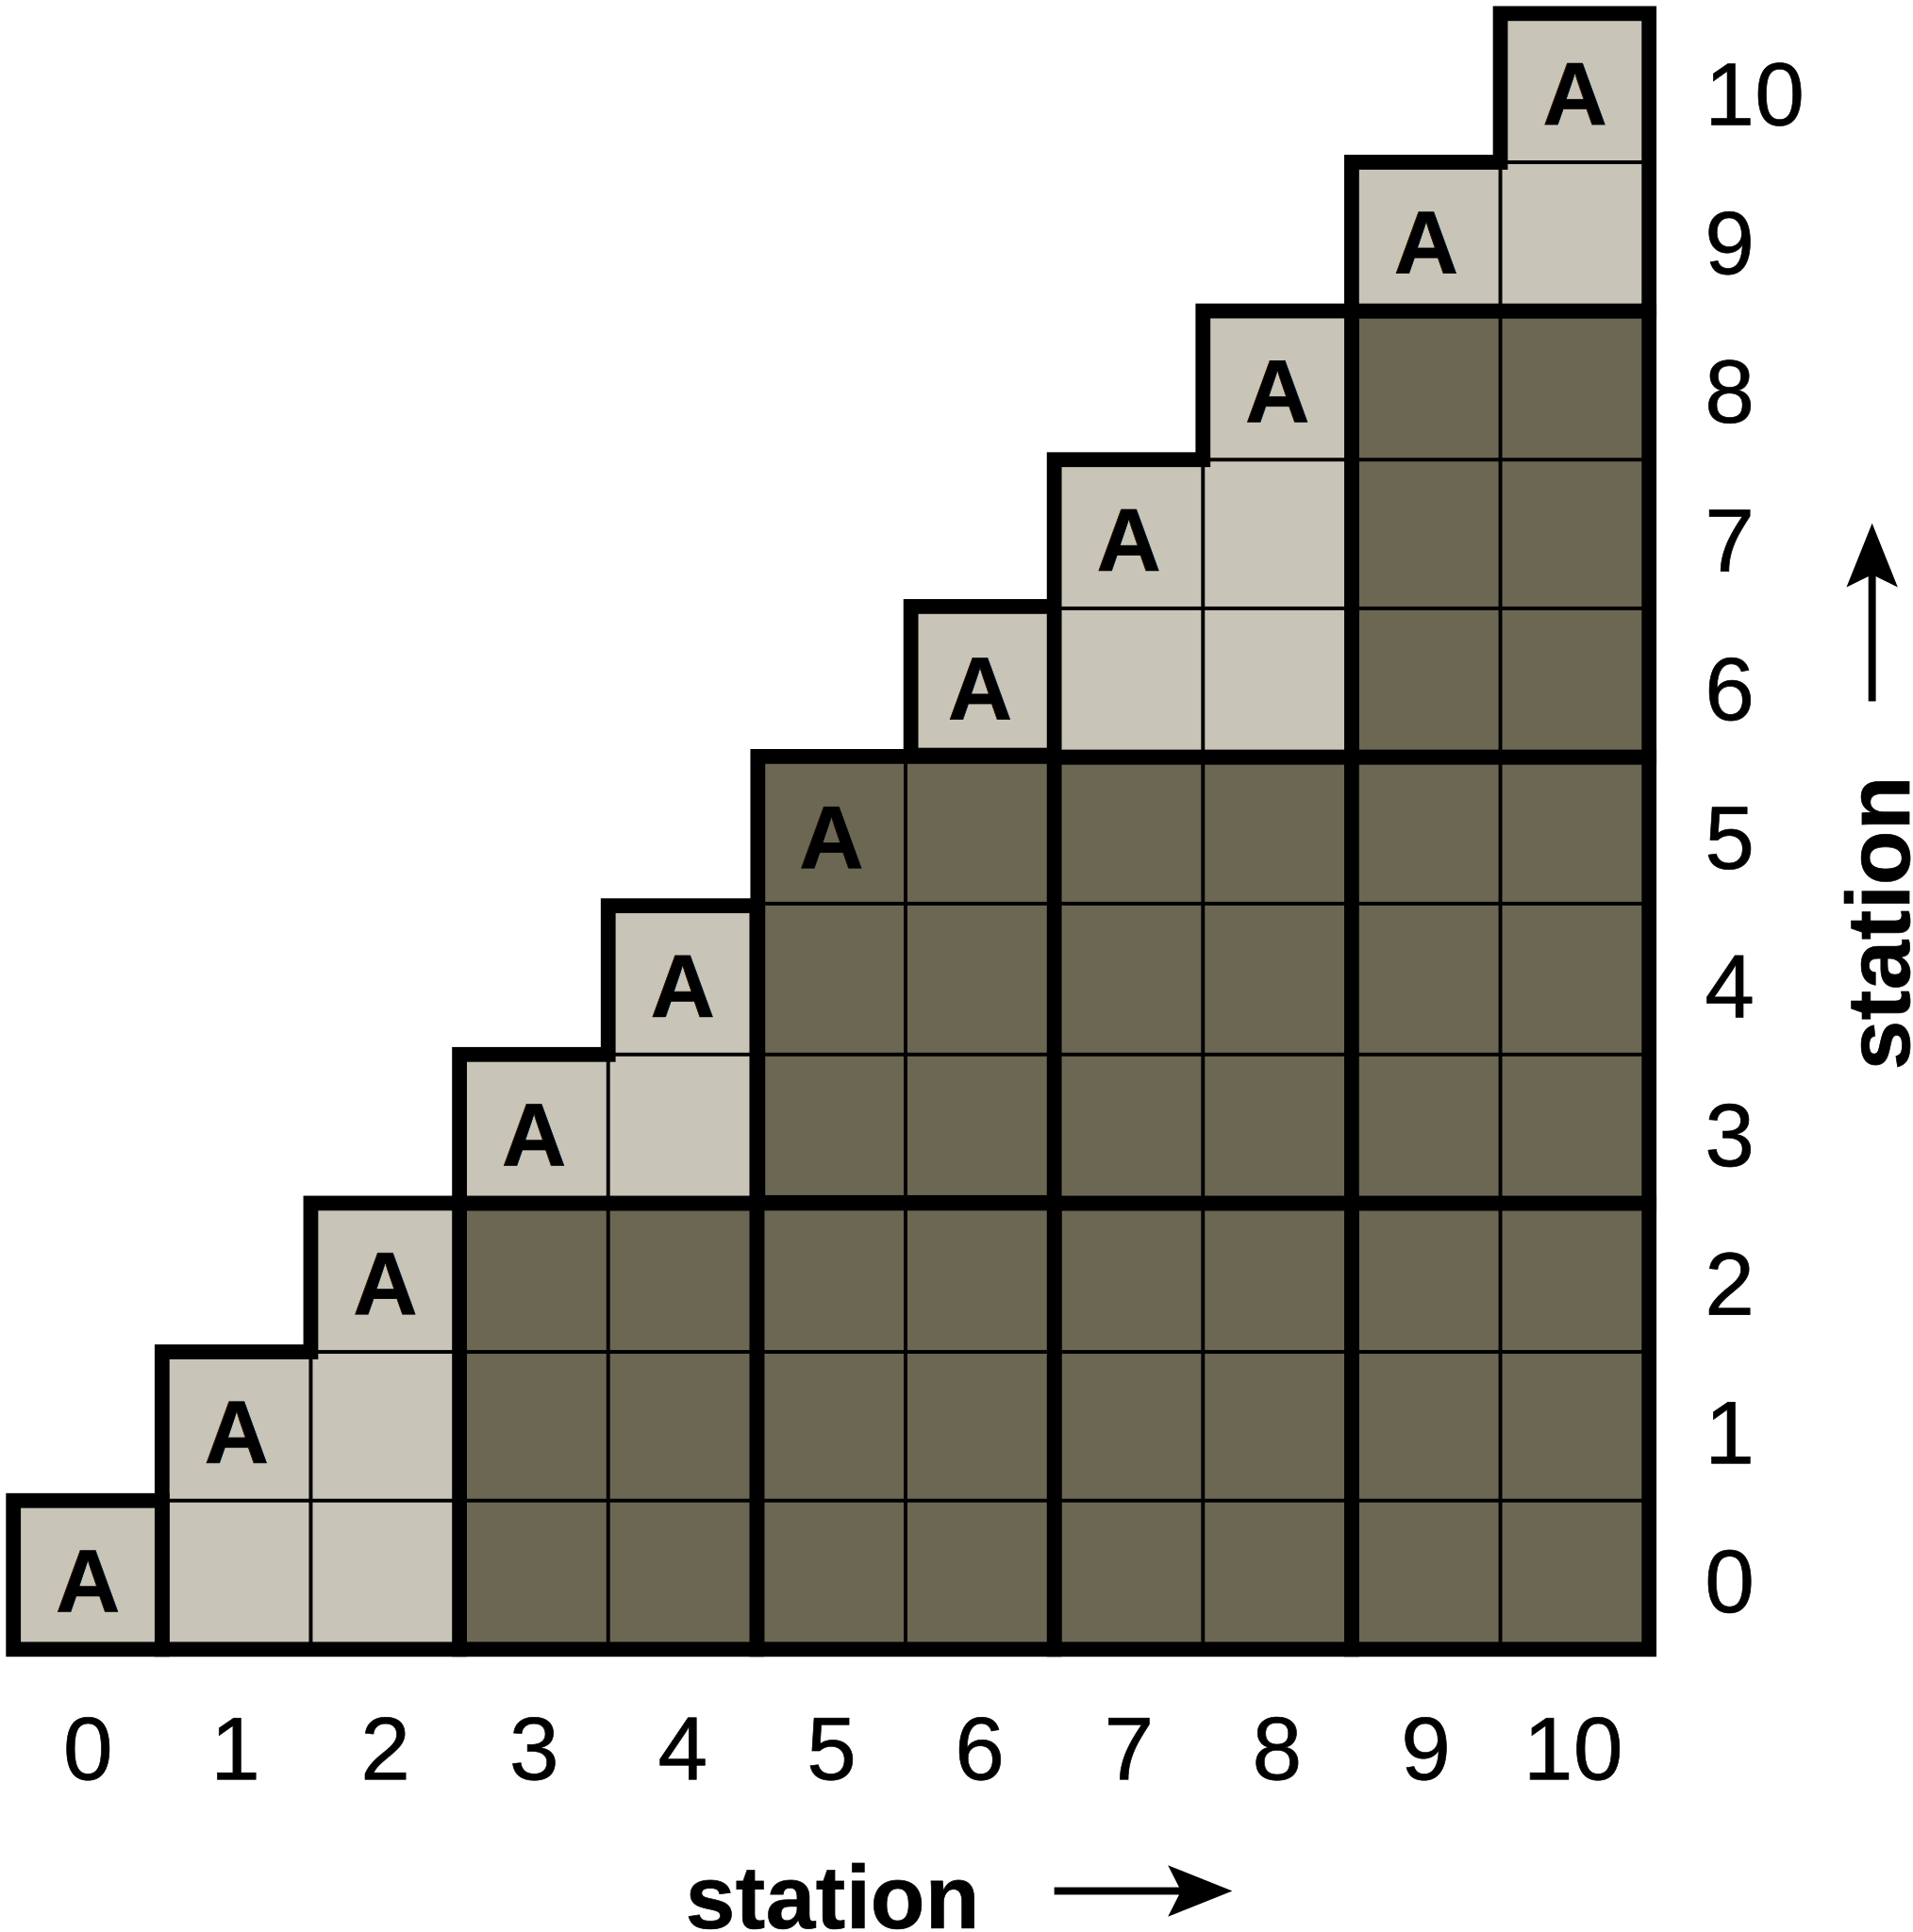
\includegraphics[width=4.2cm]{figures/correlation-triangle.pdf}
\end{center}
\vspace{-0.5cm}
\caption{An example correlation triangle.}
\label{fig-correlation}
\end{figure}

Although in reality the receivers are dual-polarized, and the samples are complex numbers, 
we use single-polarized real samples in the following example for simplicity.
An unoptimized correlator would read the samples from two receivers and
multiply them, requiring two memory loads for one multiplication.
The correlator can be optimized by reusing a sample that is read from memory
as often as possible, by using it for multiple correlations (see
Figure~\ref{fig-correlation}).
The figure is triangular, because we compute
the correlation of each pair of receivers only once. The squares labeled \emph{A} are
autocorrelations.

For example, the samples from receivers 8, 9, 10, and 11 can be correlated
with the samples from receivers 4, 5, 6, and 7 (the red square in the figure),
reusing each fetched sample four times.
This way, eight samples are read from memory for sixteen
multiplications, reducing the amount of memory operations by a factor
of four.
Correlating even higher numbers of receivers simultaneously would reduce the
memory bandwidth usage further, but the maximum number of receivers that can
be correlated this way is limited by the number of registers that an architecture has.
The accumulated correlations are also best kept in registers, and the number of
required registers grows rapidly with the number of receiver inputs.
The example above already requires 16 accumulators.
Additional registers are needed to load samples from memory (8 in this case).
To obtain good performance, it is important to tune the tile size to the
architecture.

%Caches and memory prefetch units can also improve the performance.
%However, a cache-size dependent tradeoff must be made.
%On the one hand, correlating and integrating over long periods of time
%is good for pipelined FPU operation, on the other hand, the 

There still is
opportunity for additional data reuse \emph{between} tiles.  The tiles
within a row or column in the triangle still need the same samples.
In addition to registers, caches can thus also be used to increase
data reuse. 

It is important to realize that the
correlator itself is \emph{trivially parallel}, since the tens of thousands of
frequency channels that LOFAR uses can be processed independently.  This allows us to
efficiently exploit many-core hardware.

We will now describe the implementation of the correlator on
the different architectures. 
We evaluate the performance in detail. For comparison reasons, we use the performance
\emph{per chip} for each architecture.
We choose 64 as the number of receivers (each consisting of hundreds of antennas), since
that is a realistic number for LOFAR.  Future instruments will likely
have even more receivers. The performance results are shown in Figure~\ref{performance-graph}.

\begin{figure}[t]
\begin{center}
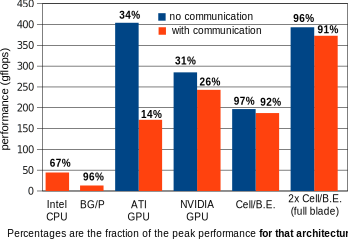
\includegraphics[width=\columnwidth]{figures/performance-graph-v2.pdf}
\end{center}
\vspace{-0.5cm}
\caption{Achieved performance on the different platforms.}
\label{performance-graph}
\end{figure}


\subsection{Intel CPUs}

We use the SSE4 instruction set to exploit vector parallelism.  Due to
the limited shuffle instructions, computing the correlations of the
four polarizations within a vector is inefficient. We achieve only a
speedup of a factor of 2.8 compared to a version without SSE4.  We
found that, unlike on the other platforms, computing four samples with
subsequent time stamps in a vector works better.  The use of SSE4
improves the performance by a factor of 3.6 in this case.  In
addition, we use multiple threads to utilize all four cores.  To
benefit from hyperthreading, we need twice as many threads as cores.  
Hyperthreading increases performance by 6\%.  The most efficient
version uses a tile size of $2 \times 2$.  Larger tile sizes are inefficient
due to the small number of SSE4 registers. 

\subsection{The BG/P supercomputer}

The LOFAR production correlator is implemented on the Blue Gene/P platform.
We use it as the reference for performance comparisons.
The (assembly) code hides load and
instruction latencies, issues concurrent floating point, integer, and
load/store instructions, and uses the L2 prefetch buffers in the most
optimal way. 
Like on the Intel CPU, we have to use a cell size of $2 \times 2$ due to
the small number of registers.
The performance we achieve with this version is 13.1 gflops per chip,
96\% of the theoretical peak performance. 
The problem is compute bound, and not I/O bound, thanks to the
high memory bandwidth per flop.
%For more information, we refer to~\cite{sc09}.

\subsection{ATI GPUs}

ATI offers two separate programming models, at different abstraction
levels.  The low-level programming model is called the ``Compute
Abstraction Layer'' (CAL).  CAL provides communication primitives and
an assembly language, allowing fine-tuning of device
performance. For high-level programming, ATI adopted \emph{Brook},
which was originally developed at Stanford~\cite{brook}. ATI's
extended version is called \emph{Brook+}~\cite{amd-manual}.  We
implemented the correlator both with Brook+ and with CAL.

With both Brook+ and CAL, the programmer has to do the vectorization,
unlike with NVIDIA GPUs.  CAL provides a feature called
\emph{swizzling}, which is used to select parts of vector registers in
arithmetic operations.  We found this improves readability of the code
significantly. However, the
programming tools still are insufficient. The high-level Brook+ model does
not achieve acceptable performance for our application. The low-level
CAL model does, but it is difficult to use.

The architecture also does not provide random write access to device
memory. The kernel output can be written to at most 8 output registers
(each 4 floats wide).  This effectively limits the
tile size to $2\times2$.  Random write access to \emph{host} memory is
provided.  The correlator reduces the data by a large amount, and the
results are never reused by the kernel. Therefore, they can be
directly streamed to host memory.

The best performing implementation uses a tile size of 4x3, thanks to
the large number of registers.  The kernel itself achieves 297 gflops,
which is 25\% of the theoretical peak performance. The performance is limited by
the device memory bandwidth.

If we also take the host-to-device transfers into account, performance
becomes much worse.  We found that the host-to-device throughput is
only 4.62 GB/s in practice, although the theoretical PCI-e bus
bandwidth is 8 GB/s.  The transfer can be done asynchronously,
overlapping the computation with host-to-device communication.
However, we discovered that the performance of the compute kernel
decreases significantly if transfers are performed concurrently.
Due to the low I/O performance, we achieve only 14\% of the theoretical peak.


\subsection{NVIDIA GPUs}

NVIDIA's programming model is called Cuda~\cite{cuda-manual}.
Cuda is relatively high-level, and achieves good performance.
However, the programmer still has to think about many details such as
memory coalescing, the texture cache, etc.
An advantage of NVIDIA hardware and Cuda is that the application does not have to do 
vectorization. This is thanks to the fact that all cores have their own address generation units. 
All data parallelism is expressed by using threads.

Since random write access to
device memory is supported (unlike with the ATI hardware), we can
simply store the output correlations to device memory.  We use the
texture cache to speed-up access to the sample data. We do not use it for the
output data, since that is written only once, and never read back by the kernel. 
With Cuda, threads
within a thread block can be synchronized.  We exploit this feature to let
the threads that access the same samples run in lock step.  This way,
we pay a small synchronization overhead, but we can increase the cache hit
ratio significantly.  We found that this optimization improved performance by a factor of 2.

We also investigated the use of the per-multiprocessor shared memory as an
application-managed cache.  Others report good results with this
approach~\cite{gpu-cache}.  However, we found that, for our
application, the use of shared memory only led to performance
degradation.

The best performing
implementation uses a tile size of 3x2.
The optimal tile size is influenced by the way the available registers are used.
The register file is a shared resource. A smaller tile size means less register usage, 
which allows the use of more concurrent threads, hiding load delays.
On NVIDIA hardware, we found that the using a relatively small tile size and many threads increases performance.

The kernel itself, without host-to-device communication achieves 31\%
of the theoretical peak performance.  If we include communication, the
performance drops to 26\% of the peak. Just like with the ATI
hardware, this is caused by the low PCI-e bandwidth.  With NVIDIA
hardware and our data-intensive kernel, we do see significant
performance gains by using asynchronous I/O.


\subsection{The Cell Broadband Engine}

The basic \mbox{Cell/B.E.} programming is based on multi-threading:
the PPE spawns threads that execute asynchronously on SPEs.
The SPEs can
communicate with other SPEs and the PPE, using mechanisms like signals and mailboxes
for synchronization and small amounts of data, or DMA transfers for
larger data.  With the \mbox{Cell/B.E.} it is important to exploit all levels of parallelism.
Applications deal with task and data parallelism across multiple SPEs, vector parallelism
inside the SPEs, and double or triple-buffering for DMA
transfers~\cite{cell}.  The \mbox{Cell/B.E.} can be
programmed in C or C++, while using intrinsics to exploit vector
parallelism.

The large number of registers allows a big tile size of 
$4\times3$, leading to a lot of data reuse.
We exploit the vector parallelism of the \mbox{Cell/B.E.} by computing the four
polarization combinations in parallel.  We found that this performs
better than vectorizing over the integration time.  This is thanks to the \mbox{Cell/B.E.}'s
excellent support for shuffling data around in the vector registers.
The shuffle instruction is executed
in the odd pipeline, while the arithmetic is executed in the even
pipeline, allowing them to overlap.

A distinctive property of the architecture is that cache transfers are
explicitly managed by the application, using DMA. This is unlike other 
architectures, where caches work transparently.
By dividing the
integration time into smaller intervals, we can keep the sample data
for \emph{all stations} in the local store.  
Because of this, we have to load and store the correlations to main
memory several times, since the sub-results have to
be accumulated.  
We overlap communication with computation, by using multiple buffers.
For the sample data we use double buffering.
Since the correlations are both read and written, we use triple buffering in this case.
Thanks to the explicit cache,
the correlator implementation fetches each sample from main memory
\emph{only exactly once}. 
Although issuing explicit DMA commands complicates programming,
for our application this is not problematic.

Due to the high
memory bandwidth and the ability to reuse data, we achieve 92\% of the peak
performance on one chip.  If we use both chips in the cell blade, we still achieve
91\%.  Even though the memory
bandwidth per operation of the \mbox{Cell/B.E.} is eight times lower than
that of the BG/P, we still achieve excellent performance, thanks to
the high data reuse factor.


\section{Comparison and Evaluation}
\label{sec:perf-compare}

\begin{table*}[t]
\begin{center}
{\footnotesize
\begin{tabular}{l|l|l|l|l}
Intel Core i7 920            & IBM Blue Gene/P                  & ATI 4870                     & NVIDIA Tesla C1060           & STI  Cell/B.E.                \\
\hline
+ well-known                 & + L2 prefetch unit               & + largest number of cores    & + random write access        & + explicit cache              \\
- few registers              & + high memory bandwidth          & + swizzling support          & + Cuda is high-level         & + random write access         \\
- no fma instruction         & - double precision only          & - low PCI-e bandwidth        & - low PCI-e bandwidth        & + shuffle capabilities        \\
- limited shuffling          & - expensive                      & - transfer slows down kernel &                              & + power efficiency            \\
                             &                                  & - no random write access     &                              & - multiple parallelism levels \\
                             &                                  & - bad Brook+ performance     &                              &                               \\
                             &                                  & - CAL is low-level           &                              &                               \\
                             &                                  & - not well documented        &                              &                               \\
\end{tabular}
} %\small
\end{center}
\vspace{-0.5cm}
\caption{Strengths and weaknesses of the different platforms for signal processing applications.}
\label{architecture-results-table}
\end{table*}

Figure~\ref{performance-graph} shows the performance on all
architectures we evaluated. The NVIDIA GPU achieves the highest
\emph{absolute} performance. Nevertheless, the GPU \emph{efficiencies}
are much lower than on the other platforms.  The \mbox{Cell/B.E.}
achieves the highest efficiency of all many-core architectures, close
to that of the BG/P. Although the theoretical peak performance of the
\mbox{Cell/B.E.} is 4.6 times lower than the NVIDIA chip, the absolute
performance is only slightly less.  If both chips in the QS21 blade
are used, the \mbox{Cell/B.E.} also has the highest absolute
performance. For the GPUs, it is possible to use more than one chip as
well, for instance with the ATI 4870x2 device. However, we found that this does not help, since the
performance is already limited by the low PCI-e throughput, and the
chips have to share this resource.
The graph indeed shows that the
host-to-device I/O has a large impact on the GPU performance, even when using one chip.  With
the \mbox{Cell/B.E.}, the I/O (from main memory to the Local Store) only has a very small impact.

In Table~\ref{architecture-results-table} we summarize the
architectural strengths and weaknesses that we identified.  Although
we focus on the correlator application in this paper, the
results are applicable to signal processing applications in
general.


\section{Programmability of the platforms}

The performance gap between assembly and a high-level programming language 
is quite different for the different platforms. It also
depends on how much the compiler is helped by manually unrolling
loops, eliminating common sub-expressions, the use of register variables,
etc., up to a level that the C code becomes almost as low-level as assembly
code. The difference varies between only a few percent to a factor of 10. 

For the BG/P, the performance from compiled C++ code was by far not
sufficient. The assembly code is approximately 10 times faster.
For both the Cell/B.E. and the Intel core~i7, we found that
high-level code in C or C++ in combination with the use of intrinsics
to manually describe the SIMD parallelism yields acceptable
performance compared to optimized assembly code.  Thus, the programmer
specifies which instructions have to be used, but can typically leave
the instruction scheduling and register allocation to the compiler.
On NVIDIA hardware, the high-level Cuda model delivers excellent
performance, as long as the programmer helps by using SIMD data types
for loads and stores, and separate local variables for values that
should be kept in registers. With ATI hardware, this is different.  We
found that the high-level Brook+ model does not achieve acceptable
performance compared to hand-written CAL code.  Manually written assembly 
is more than three times faster. Also, the Brook+ documentation is insufficient.

\longversion{
\section{Aplying the techniques: a case study with the Intel Larrabee}

Intel recently disclosed some details about the upcoming Larrabee processor,
a fully programmable GPU based on the well-known x86 instruction set.
Although performance details are unknown, it is interesting to compare the
Larrabee to the aforementioned architectures, and to see how a correlator
should be implemented to obtain optimal performance.

The processing power comes from Larrabee's relatively long vector size:
a vector holds 16~elements, where the other architectures have vectors lengths
of at most~4.
The long vector size forces us to reconsider our parallelization strategy.
There are several options to perform 16~simultaneous FMAs.
One option is to operate on 16~samples with consecutive time stamps.
A minor drawback is that the data must be ``horizontally'' added to integrate,
but this can be done outside the main loop.
Another option is to operate on samples from 16~consecutive frequencies.
%% An advantage of this may be that the input is in the right order (i.e.,
%% the 16~values can be read from consecutive memory locations) if a Poly-Phase
%% Filter precedes the correlator: the FFT outputs consecutive frequencies into
%% consecutive memory locations.
%% Both 

Another option is to correlate samples from different receivers as illustrated
by Figure~\ref{fig-correlation}.
This method minimizes memory loads, but requires additional shuffling of data.
Unfortunately, the most efficient method can only be determined empirically,
when the hardware is available.
} % end of \longversion

\section{Conclusions}
\label{conclusions}
Current and future telescopes have high computational and I/O demands.
Therefore, we evaluated the performance of the extremely
data-intensive correlator algorithm on today's many-core
architectures. This research is an important pathfinder for future
radio-astronomy instruments. We also presented general insights on how to use many-core
platforms for signal processing applications.

The many-core architectures have a significantly lower memory
bandwidth \emph{per operation} compared to traditional architectures.
Minimizing the number of memory loads per operation is of key
importance.  We do this by extensively optimizing algorithms for each
architecture.  This includes making optimal use of caches and
registers.  A high memory bandwidth per flop is not strictly
necessary, as long as the architecture (and the algorithm) allows efficient data reuse.
This can be achieved through caches, local stores and registers.

Only two architectures perform well with our correlator application.  The BG/P
supercomputer achieves high efficiencies thanks to the high memory
bandwidth per FLOP.  The \mbox{Cell/B.E.} also performs excellently,
even though its memory bandwidth per operation is eight times lower.
We achieve this by exploiting the application-managed cache and the
large number of registers, optimally reusing all sample data.
The GPUs achieve low efficiencies, party due to the low device memory bandwidth per core,
but mostly due to the low PCI-express bandwidth.

It is clear that application-level control of cache behavior (either
through explicit DMA or thread synchronization) has a substantial
performance benefit, and is of key importance for signal processing
applications.  The results also demonstrated that, for signal
processing applications, the recent trend of increasing the number of
cores does not work if I/O is not scaled accordingly.


%% \section*{Acknowledgments}
%% This work was performed in the context of the NWO STARE
%% AstroStream project.  We gratefully acknowledge NVIDIA, and in
%% particular Dr. David Luebke, for providing freely some of the GPU
%% cards used in this work. 

\bibliographystyle{IEEEbib}
\bibliography{spm}

\end{document}
